\documentclass[a4paper]{article}

% Use these
%\usepackage{times}
%\usepackage{helvet}
%\usepackage{courier}
%\usepackage{graphicx}
%\usepackage{epsfig}
%\usepackage{subfigure}
%\usepackage{enumerate}
%\usepackage{pdfpages}
%\usepackage{float}
%\usepackage{xspace}

%% Use these
\usepackage{tikz}
\usetikzlibrary{arrows,decorations.pathmorphing,backgrounds,positioning,fit}
\usetikzlibrary{shadows}
\usepackage{pgflibraryshapes}

%% Allow page margins to be changed for specified block
\def\changemargin#1#2{\list{}{\rightmargin#2\leftmargin#1}\item[]}
\let\endchangemargin=\endlist 

%% Set fbox defaults
\setlength\fboxsep{5pt}

%% Begin
\title{BDI-Learning Discussion Paper:\\ A Mobile Storage Agent}

\author{
Dhirendra Singh\\ 
dhirendra.singh@rmit.edu.au\\
}

\begin{document}

\date{3 July 2009}

\maketitle

%%
\section{Background}

Electrification of the transportation sector is currently high on the agenda for policy makers for several reasons including reducing our dependence on oil and the potential for significantly reducing greenhouse gas emissions. Plug-in Hybrid Electric Vehicles (PHEVs) are deemed a plausible solution towards this goal and several studies are currently underway to understand the implications for battery technology \cite{burke2007batte}, vehicle design \cite{bradley2009desig}, the electricity network \cite{lund2008integ}, the wider economics \cite{wellinghoff2009the-c}, and the environment \cite{samaras2008life-}. In Australia, plans are already underway for the deployment of an electric vehicle (EV) network powered by renewable energy \cite{release2008bette}. 

The battery charge of PHEVs opens the possibility for their use as distributed fast-acting energy sources that could be integrated into the electricity grid to provide demand and peak management services. Furthermore, integrated PHEVs would be especially suited for balancing renewable energy sources like wind and solar that have inherently variable output patterns.

\section{Motivating Scenario}

In this application, we evaluate an agent-based approach to mobile storage management (MSA) for a PHEV in a single-user scenario.


[Scenario picture here..]

\begin{itemize}

\item The scenario consists of one PHEV with a single user that makes daily predictable journeys between home and work during the weekdays and one trip to the shops on the weekend.

\item There are charge points at all destinations however the PHEV has a choice to charge from the electricity grid or from a renewable source (wind or solar) where available.

\item The choice of renewable for charging depends on the available output from the renewable source that may not be predictable for any given day.

\item There are discharge points at each location where the battery may be connected as a negative load to the regular circuit, but it cannot add directly to the renewable output.

\item Charging and discharging has a fixed (but different) rate of flow and may take several hours to achieve.

\item The PHEV gets charged a fee for charging (Consumption tariff), and gets paid for providing energy (Feed-in Tariff). Different rates apply for different locations. Feed-in Tariff is always higher than Consumption Tariff at every location.

\item Connection and disconnection to/from charge points at each location are considered separate procedures due to differences in the physical location of the points in relation to the parked PHEV.

\item The PHEV is fitted with a wireless receiver that is used by the network to send supply requests as well as demand data.

\item A commenced charge or discharge operation may fail due to a user access, for instance when accessing the PHEV for commuting.


\end{itemize}

The goals of the MSA are to \footnote{There is no requirement to address peak network load for the initial system. This may be introduced later to experiment with multiple MSAs.}
:
\begin{enumerate}
\item Ensure that the PHEV always has sufficient charge for any planned trips and enough surplus for N extra kms on any given day.
\item Optimise the battery charge and discharge patterns where each operation may potentially take several hours.
\item Optimise the running costs of the PHEV by considering the Feed-in and Consumption Tariffs at various locations.
\end{enumerate}

\section{Mobile Storage Agent Design}

Towards this effort we employ the Belief-Desire-Intention (BDI) \cite{rao1995bdi-a} model of agency, that lends itself well to autonomous agent systems. 

The BDI model of agency is based on the premise that all agents have \textit{beliefs} that capture the state of their world, \textit{desires} that represents the set of possible goals, and \textit{intentions} that represent the selected course of action as a result of deliberation. A BDI agent achieves its goals by executing \textit{plans}. If however, a change in the situation means that a goal cannot be fulfilled or becomes invalid, the agent aborts the current plan and deliberates once again to select a different plan based on the new situation. This adaptability makes BDI a practical choice for dynamic real world applications of agent technology.

Within the BDI framework then, achieving the MSA goals is reduced to making the correct plan choices in the correct context. We choose to use decision trees to learn these plan context conditions.

BDI is suited to our scenario for several reasons. Firstly, it allows our agents to easily adopt, suspend, resume or drop plans based on a changing context. This is necessary to manage the learning and related exploration process and to easily switch attention when a supply request is received from the network. Secondly, the BDI framework provides for meta-level planning to control the plan selection process. This enables us to easily incorporate a heuristic to supplement the decision tree network to provide higher level reasoning. Finally, the BDI plan library gracefully handles changes within the environment, thereby lending the agents towards a truly deployable solution.

For the initial system, we will disregard the running cost optimisation and focus only on optimising the battery usage for the user commutes. Figure \ref{fig:msa-gptree}  shows a possible Goal/Plan Hierarchy for a BDI agent that achieves this goal.


\begin{figure}[htbp]
\begin{changemargin}{-1.7in}{-1.7in}
\begin{center}
\fbox{
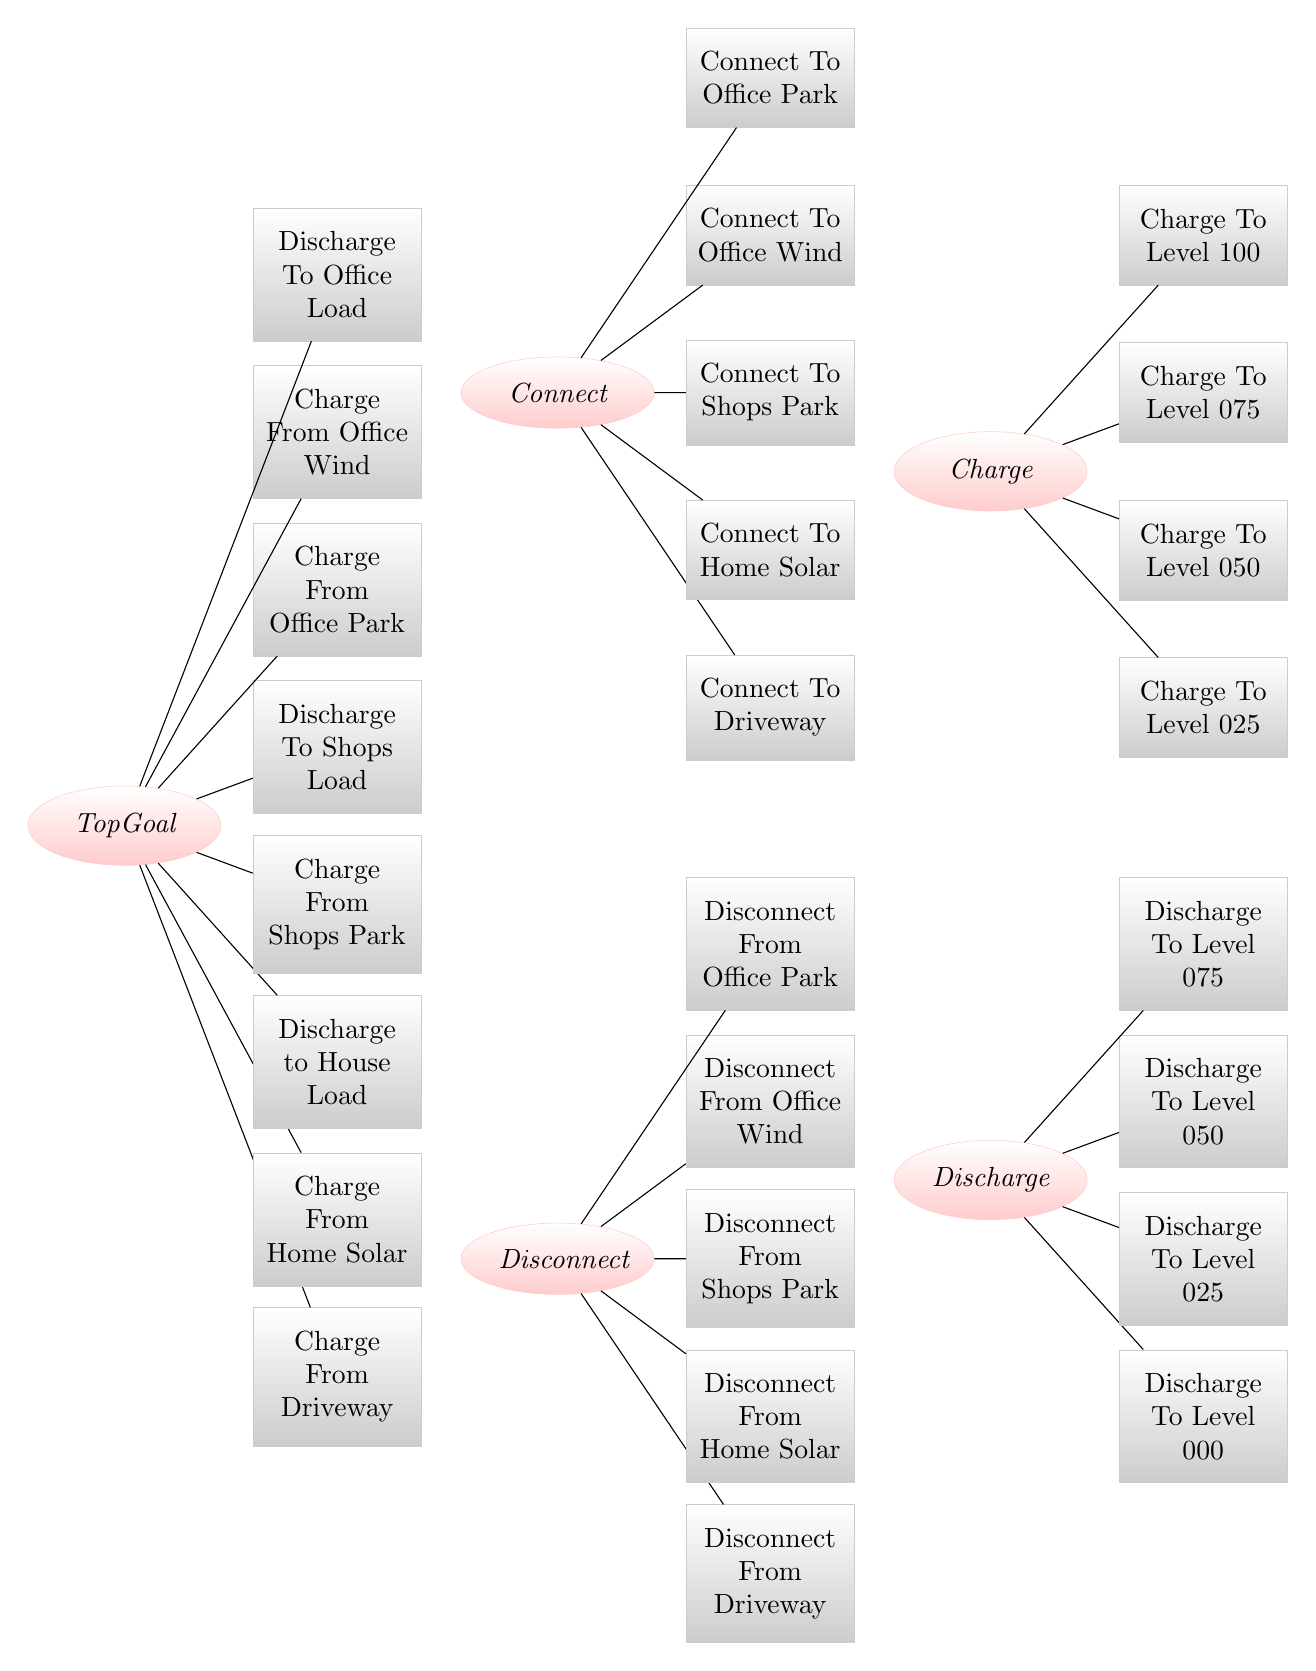
\begin{tikzpicture}
[
level distance=27mm, 
level 1/.style={sibling distance=20mm}, 
level 2/.style={sibling distance=12mm}, 
level 3/.style={sibling distance=12mm},
goal/.style={ellipse, very thin, draw=red!20, top color=white, bottom color=red!20, inner ysep=2mm, text width=15mm, text centered, font=\itshape},
plan/.style={rectangle, very thin, draw= black!20, top color=white, bottom color=black!20, inner ysep=3mm, text width=19mm, text centered}
] 
\node[goal] at (0,0) {TopGoal} [grow=right]
	child {node[plan] {Charge From Driveway}}
	child {node[plan] {Charge From Home Solar}}
	child {node[plan] {Discharge to House Load }} 
	child {node[plan] {Charge From Shops Park}}
	child {node[plan] {Discharge To Shops Load}}
	child {node[plan] {Charge From Office Park}}
	child {node[plan] {Charge From Office Wind}}
	child {node[plan] {Discharge To Office Load}
}; 
\node[goal]  at (5.5,5.5) {Connect} [grow=right]
	child {node[plan] {Connect To Driveway}}
	child {node[plan] {Connect To Home Solar}}
	child {node[plan] {Connect To Shops Park}}
	child {node[plan] {Connect To Office Wind}}
	child {node[plan] {Connect To Office Park}
};

\node[goal]  at (11,4.5) {Charge} [grow=right]
	child {node[plan] {Charge To Level 025}}
	child {node[plan] {Charge To Level 050}}
	child {node[plan] {Charge To Level 075}}
	child {node[plan] {Charge To Level 100}
};

\node[goal]  at (11,-4.5) {Discharge} [grow=right]
	child {node[plan] {Discharge To Level 000}}
	child {node[plan] {Discharge To Level 025}}
	child {node[plan] {Discharge To Level 050}}
	child {node[plan] {Discharge To Level 075}
};

\node[goal]  at (5.5,-5.5) {Disconnect} [grow=right]
	child {node[plan] {Disconnect From Driveway}}
	child {node[plan] {Disconnect From Home Solar}}
	child {node[plan] {Disconnect From Shops Park}}
	child {node[plan] {Disconnect From Office Wind}}
	child {node[plan] {Disconnect From Office Park}
};
\end{tikzpicture}
}
\end{center}
\caption{BDI Goal-Plan Hierarchy for the MSA}
\label{fig:msa-gptree}
\end{changemargin}
\end{figure}

\bibliographystyle{plain}
\bibliography{ed.bib} 

\end{document}